\documentclass[UTF8, xcolor=table]{beamer}
\usepackage[BoldFont,SlantFont]{xeCJK}
\setCJKmainfont[BoldFont={Adobe Heiti Std},ItalicFont={Adobe Kaiti Std}]{AdobeSongStd-Light}
% \setCJKmainfont[BoldFont={Adobe Heiti Std},ItalicFont={Adobe Kaiti Std}]{SimSum} %Windows先编译使用这个字体

\usepackage{latexsym,amssymb,amsmath,amsbsy,amsopn,amstext,xcolor,multicol}
\usepackage{graphicx,wrapfig,fancybox}
\usepackage{pgf,pgfarrows,pgfnodes,pgfautomata,pgfheaps,pgfshade}
\usepackage{thubeamer}
\usepackage[backend=bibtex,sorting=none]{biblatex} % [参考文献格式](https://www.sharelatex.com/blog/2013/07/31/getting-started-with-biblatex.html) %mac IEEE not found
\usepackage{array}
\usepackage{bm}
\usepackage{caption}
\RequirePackage[font=footnotesize]{subcaption}
\usepackage{multirow}
\usepackage{booktabs}
\usepackage{tikz}
\usepackage{tikzscale}
\usepackage{animate}

\defbibheading{bibliography}[\bibname]{} %avoid printbibliography 自动生成目录
\addbibresource{../main.bib}
\setbeamertemplate{bibliography item}[text] 

\usepackage{boxedminipage} %for: bvh border
\def\fourgraphicswidth{0.35} %0.3\textwidth

\usepackage{algorithm} %%format of the algorithm
\usepackage{algpseudocode}
\floatname{algorithm}{算法}
\renewcommand{\algorithmicrequire}{\textbf{输入:}} % Use Input in the format of Algorithm
\renewcommand{\algorithmicensure}{\textbf{输出:}} % UseOutput in the format of Algorithm
\algrenewcommand{\algorithmiccomment}[1]{ $//$ #1}

\usepackage{listings}
\renewcommand\lstlistingname{代码}
\renewcommand\lstlistlistingname{代码}

\lstset{framexleftmargin=1.4em,
        xleftmargin=1.8em,
        basicstyle=\ttfamily\small,
        %frame=shadowbox, numberstyle=\tiny, breaklines=true,
        frame=single,
        numberstyle=\tiny, breaklines=true,
        keywordstyle=\color{blue!70}\bfseries,
        %commentstyle=\color{red!50!green!50!blue!50},
        rulesepcolor=\color{red!20!green!20!blue!20},
        numbers=none,fontadjust=true}
\lstdefinelanguage{shader}{morekeywords={uniform, layout, uniform, vec2, vec3, vec4, in, out, gl_Position, dot, flat, int ,float, gl_VertexID, xyz, w, x, y, z, location, version, sampler2DRect, bgr, gl_FragData, texture2DRect, gl_TexCoord,for,xy},morecomment=[l]{//}}

\begin{document}

\setbeamerfont{footnote}{size=\tiny}
\setbeamerfont{caption}{size=\scriptsize}
\setbeamertemplate{caption}[numbered]
\setbeamerfont{subsection in toc}{size=\footnotesize}
\renewcommand*{\bibfont}{\footnotesize}

\graphicspath{{../}}

\title[融合长短记忆神经网络与卷积特征学习的图像语义分割]{中山大学本科毕业论文演示文稿非正式模版}
\author[陈冠英]{}%{(申请中山大学工学学士学位论文答辩报告)\\ \vskip 20pt 学~~~~~~生:陈~冠~英}
\institute[中山大学~电子信息与工程学院~\&~自动化]{}%{\small \vskip 38pt 电子信息与工程学院~自动化}
\date{} %{\small \vskip -17pt二〇一六年五月}

%% make title %%
\frame{
	\titlepage
	\vspace{-23mm}
	\begin{figure}[h]
		\centering
		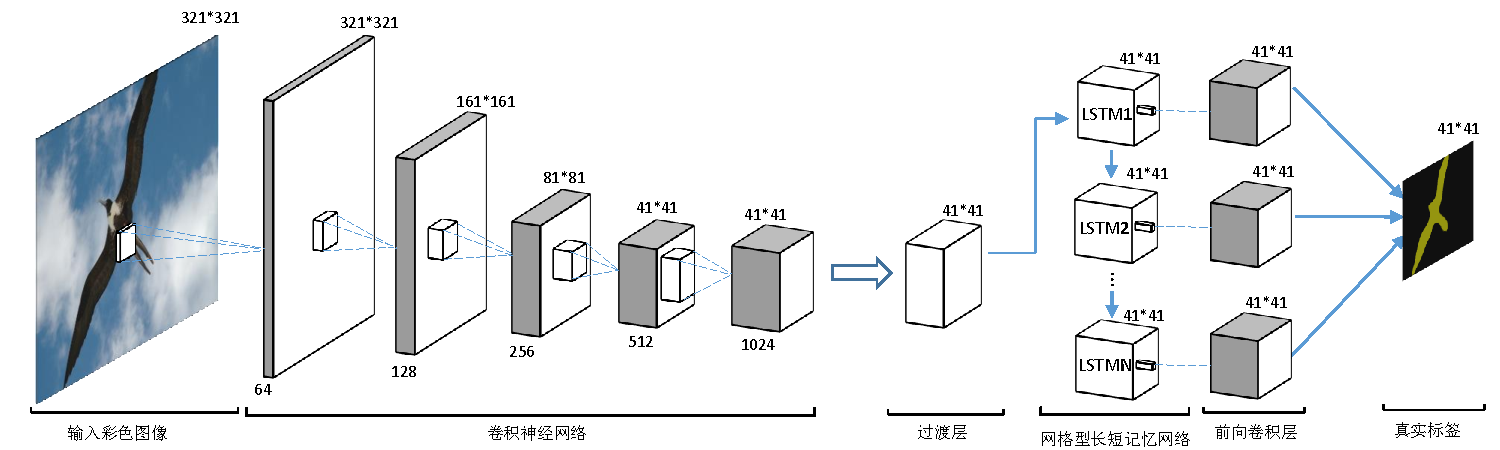
\includegraphics[width=\textwidth]{image/illustration/networkstructure.pdf}
	\end{figure}
}

\frame {
	\frametitle{目录}
	%\begin{multicols}{2}
	\tableofcontents[sections={<1-7>}]
}

\section{引言}
\frame
{
  \frametitle{\secname~ }
  \begin{block}{选题背景与意义}
	  是什么,为什么?
  \end{block}
  \begin{block}{国内外研究现状}
	  主流方法是什么?
  \end{block}
  \begin{block}{本文的工作}
	  我提出的方法是什么,有什么不同?
  \end{block}
}

\subsection*{选题背景与意义}
\frame{
  \frametitle{图像语义分割问题的定义}
  \begin{block}{}
	图像语义分割 (Semantic Image Segmentation) 是根据物体类别把图像分成若干个有意义的区域,并为不同的区域标注其所属标签的视觉任务。
  \end{block}
\begin{figure}%文中的Grid-LSTM模型做的语义图像分割的例子
	\centering
	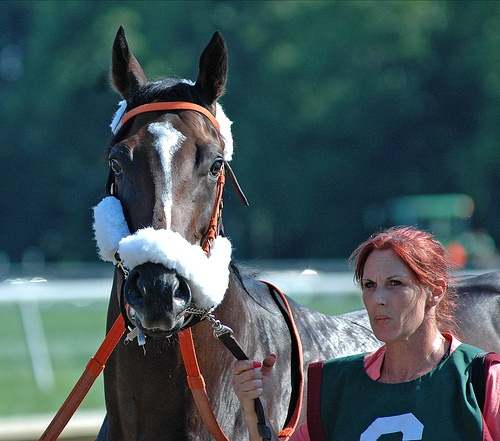
\includegraphics[width=.2\textwidth,height=.15\textwidth]{image/example/2007_000799.jpg}
	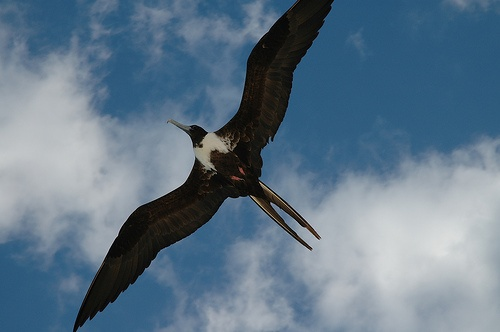
\includegraphics[width=.2\textwidth,height=.15\textwidth]{image/example/2007_002094.jpg}
	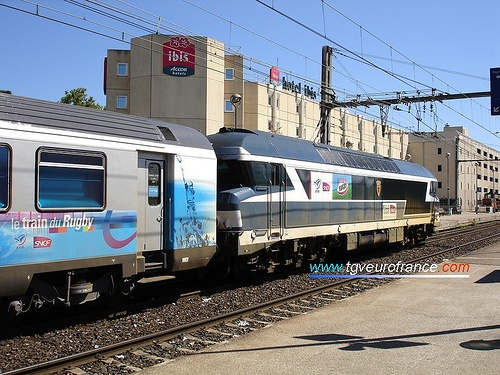
\includegraphics[width=.2\textwidth,height=.15\textwidth]{image/example/2007_004483.jpg}
	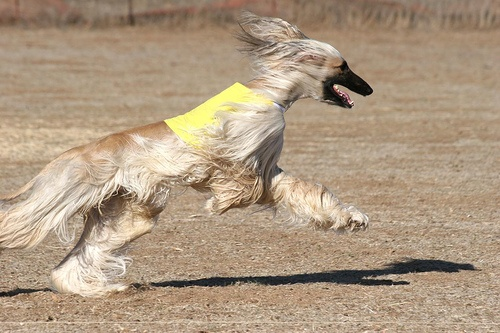
\includegraphics[width=.2\textwidth,height=.15\textwidth]{image/example/2007_003194.jpg}
	\\
	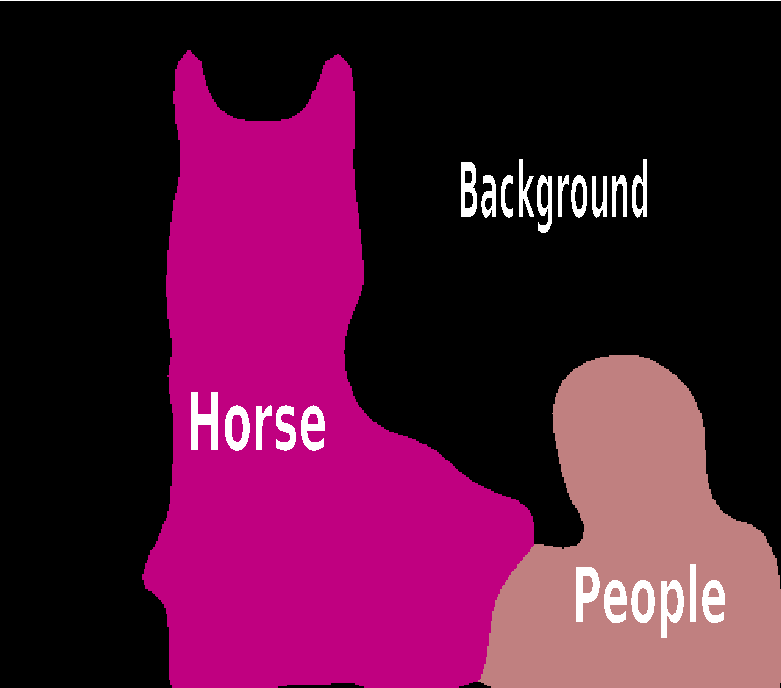
\includegraphics[width=.2\textwidth,height=.15\textwidth]{image/example/2007_000799.pdf}
	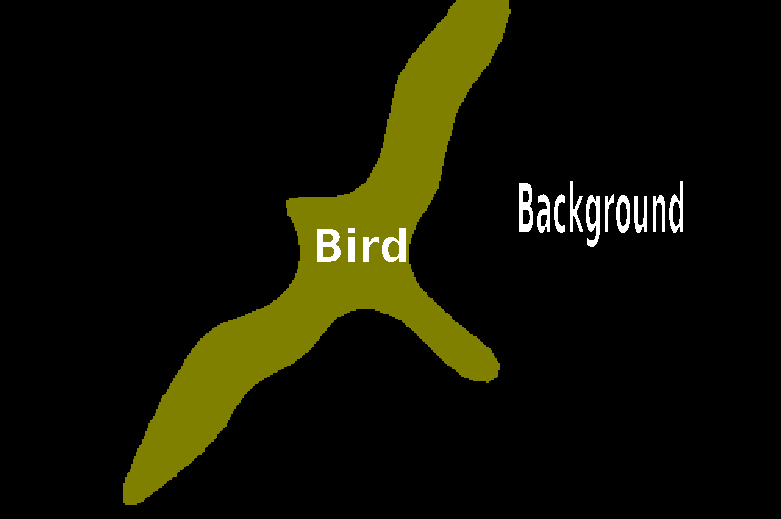
\includegraphics[width=.2\textwidth,height=.15\textwidth]{image/example/2007_002094.pdf}
	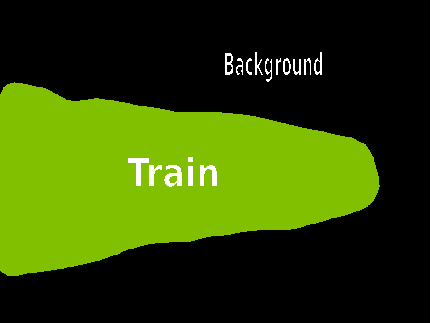
\includegraphics[width=.2\textwidth,height=.15\textwidth]{image/example/2007_004483.pdf}
	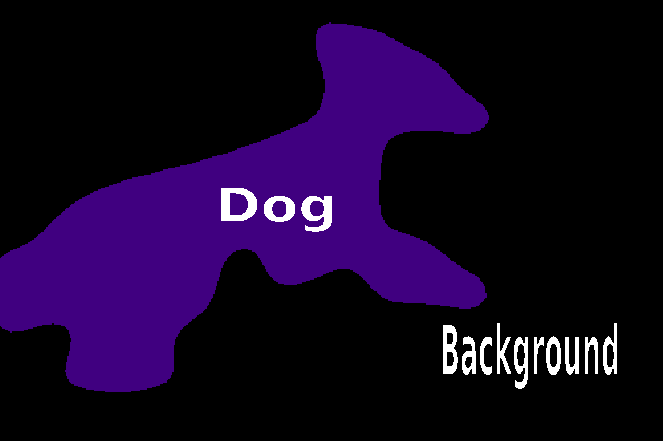
\includegraphics[width=.2\textwidth,height=.15\textwidth]{image/example/2007_003194.pdf}
	\caption[语义图像分割的例子]{本文模型在VOC 2012验证集上的语义图像分割例子}
	\label{fig:example1}
\end{figure}
}

\frame{
   \begin{block}{选题的背景}
   \begin{itemize}
	\item 手工设计特征的局限性(SIFT, HOG)
	\item 深度学习技术的兴起
		\begin{itemize}
			\item 基于GPU的并行化计算 
			\item 大型训练集的标注 
		\end{itemize}
	\item 大数据与智能时代正在来临
   \end{itemize}
   \end{block}

   \begin{block}{选题的意义}
	\begin{itemize}
		\item[\dag] 图像语义分割解决了图像里面有什么,物体的形状与位置的问题
   \end{itemize}
   \vspace{-1em}
   \begin{multicols}{2}
   \begin{itemize}
	\item 图像检索
	\item 图像编辑
	\item 现实增强
	\item 机器导航
   \end{itemize}
   \end{multicols}
   \end{block}
   \}
}
\subsection*{国内外研究现状}

\frame{
	\frametitle{主流方法中的代表性工作}
	\begin{columns}[t]
		\column{.5\textwidth}
		\centering
		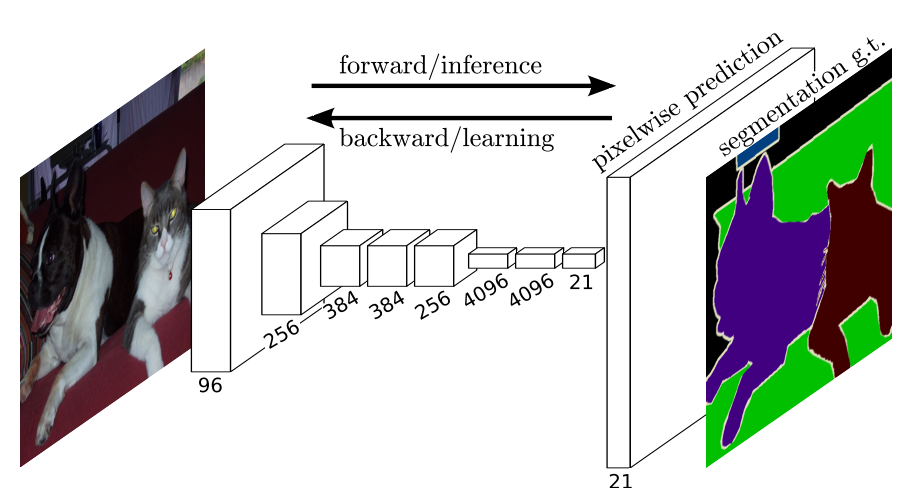
\includegraphics[width=\textwidth]{figures/FCN} \\
		\makebox[0.5\textwidth]{\tiny a. 全卷积网络[Long et al, CVPR 2015]} \\
		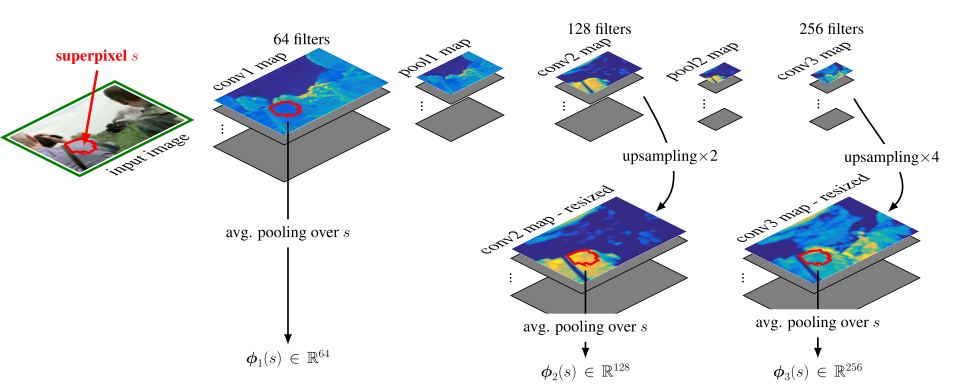
\includegraphics[width=\textwidth]{figures/zoom-out} \\
		\makebox[0.5\textwidth]{\tiny c. 卷积网络+高低层次特征融合[Mostajabi et al, CVPR 2015]} 

		\column{.5\textwidth}
		\centering
		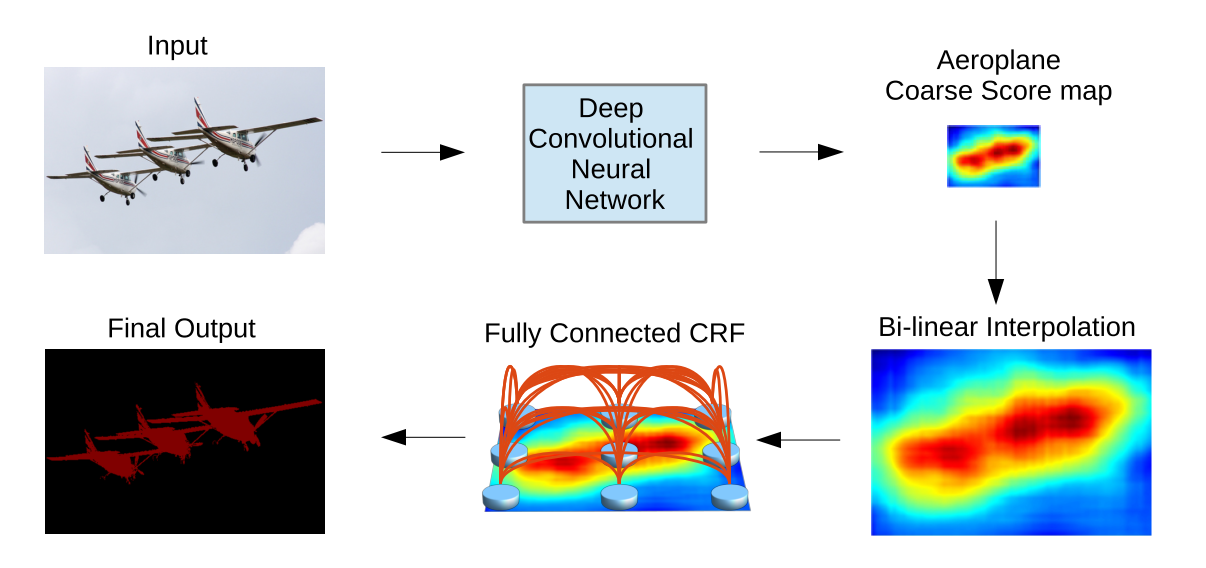
\includegraphics[width=\textwidth]{figures/Deeplab} \\
		\makebox[0.5\textwidth]{\tiny b. 全卷积网络+概率图模型[Chen et al, ICLR 2015]} \\
		\vspace{0.8em}
		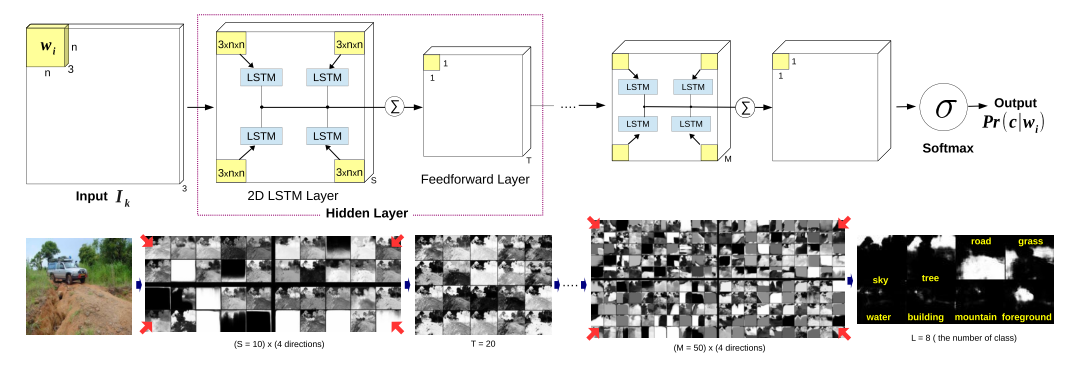
\includegraphics[width=\textwidth]{figures/LSTM} \\
		\makebox[0.5\textwidth]{\tiny d. 二维长短记忆网络[Byeon et al, CVPR, 2015]}
	\end{columns}
}
\subsection*{本文的工作}
\frame{
	\vspace{-0.6em}
	\begin{figure}[h]
		\centering
		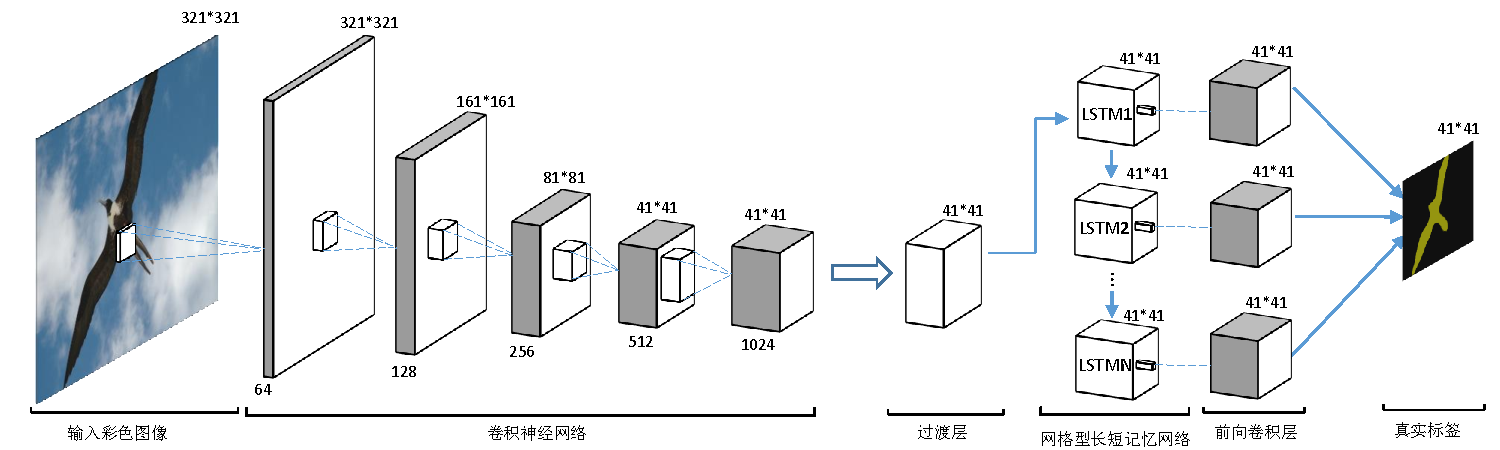
\includegraphics[width=\textwidth]{image/illustration/networkstructure.pdf}
		\caption{网络整体结构图}
	\end{figure}
	\vspace{-1.2em}
	\begin{block}{目标与思路}
		\footnotesize
	\begin{itemize}
		\item 充分利用全卷积网络强大的特征学习能力
		\item 借助长短记忆网络对特征整体与局部建模的良好能力
		\item 使用随机梯度下降法进行端到端的训练
		\item 在主流数据集验证模型有效性
	\end{itemize}
	\end{block}
}


\chapter{方案设计}
\label{cha:example}


\setmonofont [Path = fonts/] {CascadiaCode}
\newfontfamily\cyrillicfonttt [Path = fonts/] {CascadiaCode}
\newfontfamily\englishfonttt [Path = fonts/] {CascadiaCode}

\lstset{
    basicstyle = \small\ttfamily,
    tabsize=4
}

\section{课程作业目的}

本实验旨在通过对同一网络拓扑实现经典路由与基于SDN的路由,对比二者的性能差异,进而验证SDN相较于传统网络的灵活性与优越性。

\section{场景设计与预期要求}

\subsection{实验场景设计}

设计如下的小型网络拓扑进行实验:

\begin{figure}[h]
	\centering
	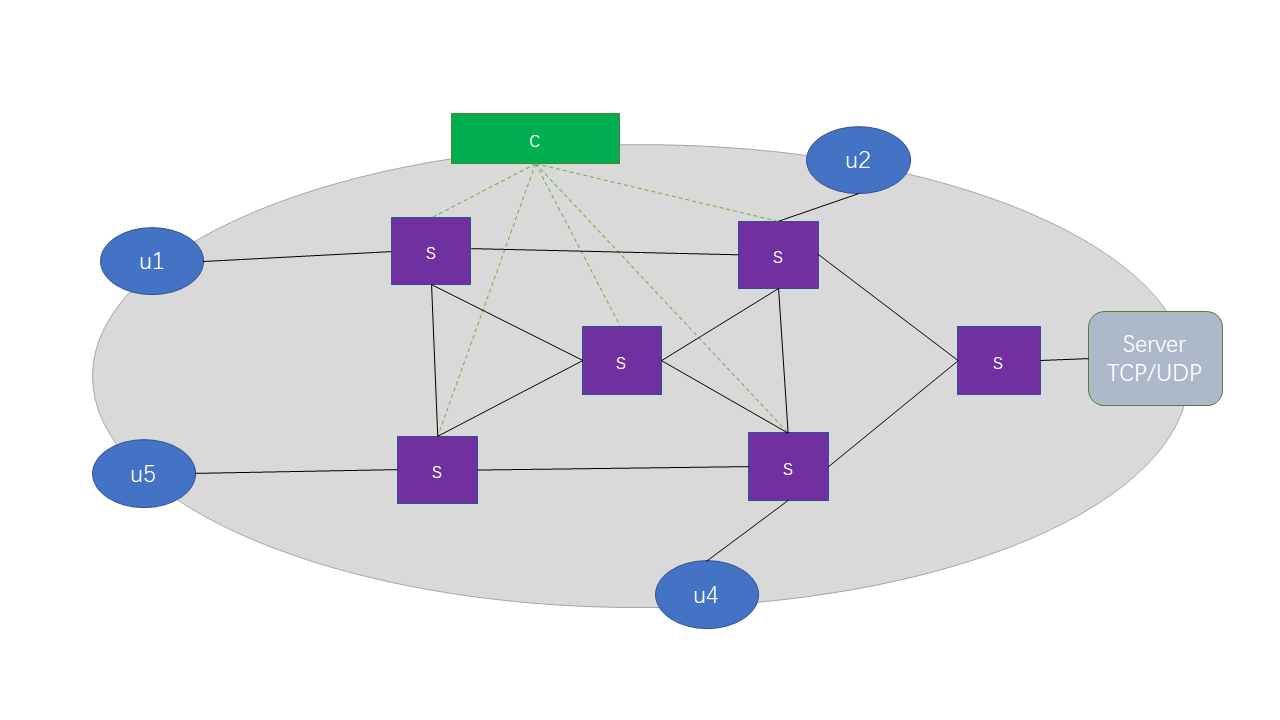
\includegraphics[width=0.9\textwidth]{image/raw_topo.png}
	\caption{实验网络拓扑}
 	\label{fig:topo}
\end{figure}

其中C为控制器,S为SDN交换机,u1-u5为终端。我们设计以下两种路由策略:

\begin{enumerate}
	\item 按目的地址路由:采用最短路径算法
	\item 按多重约束路由:目的地址+传输层协议类型(UDP通道,TCP通道)
\end{enumerate}

在测试时令u1, u5同时发送TCP/UDP流到服务器,分别在每个SDN交换机采集流量,
分析传统IP路由和SDN路由的各项QoS性能指标。

\subsection{实验预期要求}

依照上述场景设计,实验应达到如下预期要求:

\begin{itemize}
	\item 在mininet中依照实验场景搭建网络拓扑
	\item 在该拓扑上成功实现并运行按目的地址路由
	\item 在该拓扑上成功实现并运行按多重约束路由
	\item 实现一种通用的测量链路节点QoS性能指标的方法,以便对两种路由策略进行对比与评价
\end{itemize}


\section{实现方案与技术细节}

\subsection{实现方案}

\subsubsection{拓扑设计}

拓扑设计参照实验要求,实验时的拓扑如下:

\begin{figure}[h]
	\centering
	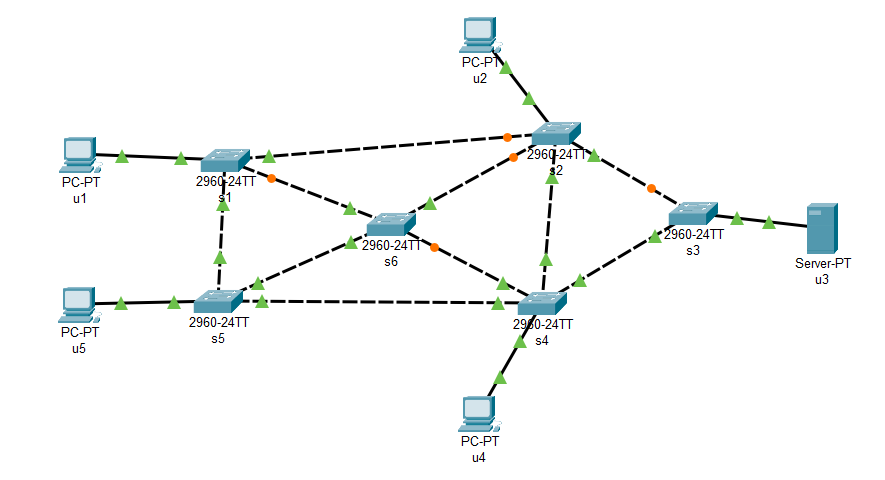
\includegraphics[width=0.9\textwidth]{../topo/topo.png}
	\caption{拓扑图}
 	\label{fig:topo2}
\end{figure}

其中,$u_{3},u_{6},u_{7},u_{8}$ 作为iperf3测试时的服务器,
$u_{1},u_{5}$作为iperf3测试时的客户端。

各链路均有带宽和延迟的参数,如下表所示:

% \usepackage{booktabs}
% \usepackage{caption}
\begin{table}

\centering
\begin{tabular}{cccccc}
  \toprule
  & $s_1 - s_2 $ & $ s_1 - s_5 $ & $s_2-s_4$ & $s_4-s_6$ & 其他 \\
  \midrule
  延迟($ms$) & 15 & 15 & 15 & 15 & 10 \\
  带宽($Mbps$) & 50 & 50 & 50 & 50 & 75 \\
  \bottomrule
\end{tabular}
\caption{延迟带宽表}
\end{table}

\subsubsection{传统路由方案设计}

使用Ryu控制器自带的 \texttt{ryu.app.rest\_router},可以进行传统的基于最短距离的路由。

\texttt{ryu.app.rest\_router}实现了两个功能:

\begin{itemize}
	\item 生成路由规则并下发给Switch。这样一来每个Switch都可以看作一个路由器。
	\item 支持通过一套Restful API对路由规则进行增删改查,这样一来外部可以根据需要修改路由规则。
\end{itemize}

但这个APP并不能自动地进行路由规则的生成,我们需要通过某种规则来生成路由并通过此APP的Restful API部署生成的路由规则。
\texttt{classic/make\_route.py}文件就实现了根据最短路径算法生成路由并告知\texttt{ryu.app.rest\_router}的过程。

主要的生成过程如下:

\begin{enumerate}
	\item 把拓扑视作一个图,通过在每个点进行Dijkstra算法生成两点之间的最短路径。
	\item 通过路径生成路由信息。
如$u_1$到$u_3$的最短路径是$u_1 \rightarrow u_2 \rightarrow u_3$,
那么生成类似于$(dst:u_3, next\_hop:u_2)$的路由信息。
	\item 把生成的路由信息发送给\texttt{ryu.app.rest\_router}
\end{enumerate}

这样的方法需要我们提前给定两个点之间的边权,这里把延迟作为边权。

\subsubsection{基于TCP与UDP路由的SDN路由方案设计}

首先给定一套把从$u_1$和$u_5$发出的TCP和UDP进行分流的方案:

\begin{figure}[h]
	\centering
	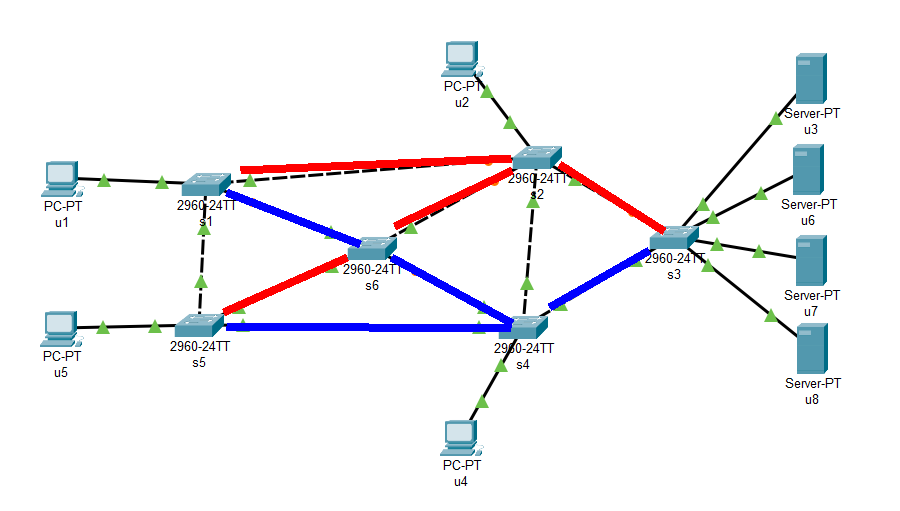
\includegraphics[width=0.9\textwidth]{image/topo_tcp_udp.png}
	\caption{UDP和TCP路径}
 	\label{fig:topo3}
\end{figure}

如图,红色路径是TCP流的路径,蓝色路径是UDP流的路径。

实现这个路径需要用到Ryu控制器自带的\texttt{ryu.app.ofctl\_rest},
这个APP提供了一套增删改查任意Switch流表的Restful API,
使用它可以方便地创建所需的流表项。

在传统路由的基础上创建几个特定的高优先级流表项即可。

\subsubsection{Qos性能测试设计}

这里采用了iperf3工具进行测试。iperf3工具可以创建一段时间的TCP和UDP通信,
这一段通信的速率、延迟、丢包等信息可以帮助我们获取Qos性能信息。
也可以在测试时实时进行报文抓取,这也反映了很多Qos性能信息。

\subsection{实现传统路由}

\subsubsection{搭建拓扑}

首先找到 \texttt{classic/create\_{}topo.py} 这个文件,
在配置好mininet的主机$A$中运行
\begin{lstlisting}
	sudo mn --custom create_topo.py --topo mytopo \
	--switch ovs --controller remote,ip={ip of B} --link tc
\end{lstlisting}

其中 \texttt{ip} 项是控制器主机$B$的 ip 地址。

在$B$主机中运行

\begin{lstlisting}
	ryu run --observe-links  \
	ryu.app.rest_router ryu.app.gui_topology.gui_topology
\end{lstlisting}

这样一来整个拓扑已经搭建成功。浏览 \texttt{http://ip\_of\_B:8080} 可以查看拓扑图像如下:

\begin{figure}[h]
	\centering
	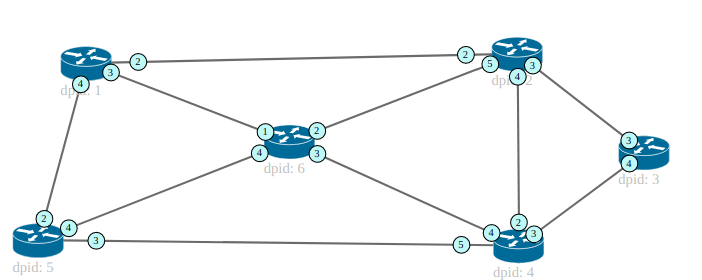
\includegraphics[width=0.5\textwidth]{image/topo1.png}
	\caption{拓扑图}
 	\label{fig:hole}
\end{figure}


注意到这里没有画出主机的拓扑情况。

\subsubsection{生成路由}

首先找到 \texttt{classic/make\_route.py},在主机$B$上运行

\begin{lstlisting}
	python make_route.py
\end{lstlisting}

这会在控制器上创建基于最短路算法的静态路由。
此时路由已经创建好,但是,由于主机的默认网关均未进行配置,要手动配置默认网关。

在mininet的命令行中运行

\begin{lstlisting}
	u1 ip route add default via 172.18.0.2 \
	u2 ip route add default via 172.18.1.2 \
	u3 ip route add default via 172.18.2.2 \
	u4 ip route add default via 172.18.3.2 \
	u5 ip route add default via 172.18.4.2 \
	u6 ip route add default via 172.18.2.2 \
	u7 ip route add default via 172.18.2.2 \
	u8 ip route add default via 172.18.2.2
\end{lstlisting}

这样一来路由就搭建成功了。

\subsubsection{测试路由}

在mininet的命令行中运行

\begin{lstlisting}
	pingall
\end{lstlisting}

得到输出如下:

\begin{lstlisting}
	mininet> pingall
	*** Ping: testing ping reachability
	u1 -> u2 u3 u4 u5 u6 u7 u8 
	u2 -> u1 u3 u4 u5 u6 u7 u8 
	u3 -> u1 u2 u4 u5 u6 u7 u8 
	u4 -> u1 u2 u3 u5 u6 u7 u8 
	u5 -> u1 u2 u3 u4 u6 u7 u8 
	u6 -> u1 u2 u3 u4 u5 u7 u8 
	u7 -> u1 u2 u3 u4 u5 u6 u8 
	u8 -> u1 u2 u3 u4 u5 u6 u7 
	*** Results: 0% dropped (56/56 received)
\end{lstlisting}

这样一来就可以确定路由已经正常工作。

\subsubsection{性能测试}

在mininet的命令行中运行

\begin{lstlisting}
	u3 iperf3 -s -D
	u6 iperf3 -s -D
	u7 iperf3 -s -D
	u8 iperf3 -s -D
	u1 iperf3 -c u3 -t 20 > u1.tcp &
	u1 iperf3 -c u6 -u -b 40M > u1.udp &
	u2 iperf3 -c u7 -t 20 > u2.tcp &
	u2 iperf3 -c u8 -u -b 40M > u2.udp &
\end{lstlisting}

性能测试的结果在 \texttt{u1.tcp, u1.udp, u2.tcp, u2.udp} 这四个文件中。

\subsection{实现基于UDP和TCP选择的SDN路由}

\subsubsection{搭建拓扑}

首先找到 \texttt{classic/create\_{}topo.py} 这个文件,
在配置好mininet的主机$A$中运行
\begin{lstlisting}
	sudo mn --custom create_topo.py --topo mytopo \
	--switch ovs --controller remote,ip={ip of B} --link tc
\end{lstlisting}

其中 \texttt{ip} 项是控制器主机$B$的 ip 地址。

在$B$主机中运行

\begin{lstlisting}
	ryu run --observe-links  \
	ryu.app.rest_router ryu.app.gui_topology.gui_topology \
	ryu.app.ofctl_rest
\end{lstlisting}

这样一来整个拓扑已经搭建成功。实际上,这里的拓扑和传统路由时的拓扑没有区别。

\subsubsection{生成路由}
首先找到 \texttt{sdn-tcp-udp} 文件夹中的 
\texttt{make\_classic\_route.py}和
\texttt{make\_sdn\_route.py},
在主机$B$上运行

\begin{lstlisting}
	python make_classic_route.py \
	python make_sdn_route.py
\end{lstlisting}

这会在控制器上创建基于最短路算法的静态路由和基于UDP和TCP的SDN路由。

此时路由已经创建好,但是,由于主机的默认网关均未进行配置,要手动配置默认网关。

在mininet的命令行中运行

\begin{lstlisting}
	u1 ip route add default via 172.18.0.2 
	u2 ip route add default via 172.18.1.2
	u3 ip route add default via 172.18.2.2
	u4 ip route add default via 172.18.3.2
	u5 ip route add default via 172.18.4.2
	u6 ip route add default via 172.18.2.2
	u7 ip route add default via 172.18.2.2
	u8 ip route add default via 172.18.2.2
\end{lstlisting}

这样一来路由就搭建成功了。

\subsubsection{测试路由}

在mininet的命令行中运行

\begin{lstlisting}
	pingall
\end{lstlisting}

得到输出如下:

\begin{lstlisting}
	mininet> pingall
	*** Ping: testing ping reachability
	u1 -> u2 u3 u4 u5 u6 u7 u8 
	u2 -> u1 u3 u4 u5 u6 u7 u8 
	u3 -> u1 u2 u4 u5 u6 u7 u8 
	u4 -> u1 u2 u3 u5 u6 u7 u8 
	u5 -> u1 u2 u3 u4 u6 u7 u8 
	u6 -> u1 u2 u3 u4 u5 u7 u8 
	u7 -> u1 u2 u3 u4 u5 u6 u8 
	u8 -> u1 u2 u3 u4 u5 u6 u7 
	*** Results: 0% dropped (56/56 received)
\end{lstlisting}

这样一来就可以确定路由已经正常工作。

\subsubsection{性能测试}

这里进行了两次性能测试,一次测试和传统路由相同,限制udp的速率为$40 Mbp/s$,
一次把udp的速率限制到$100 Mbp/s$。

在mininet的命令行中运行

\begin{lstlisting}
	u3 iperf3 -s -D
	u6 iperf3 -s -D
	u7 iperf3 -s -D
	u8 iperf3 -s -D

	u1 iperf3 -c u3 -w 1M -t 20 > u1-40.tcp &
	u1 iperf3 -c u6 -u -b 40M > u1-40.udp &
	u5 iperf3 -c u7 -w 1M -t 20 > u5-40.tcp &
	u5 iperf3 -c u8 -u -b 40M > u5-40.udp &

	u1 iperf3 -c u3 -w 1M -t 20 > u1-100.tcp &
	u1 iperf3 -c u6 -u -b 100M > u1-100.udp &
	u5 iperf3 -c u7 -w 1M -t 20 > u5-100.tcp &
	u5 iperf3 -c u8 -u -b 100M > u5-100.udp &
\end{lstlisting}

第一次性能测试的结果在 \texttt{u1-40.tcp, u1-40.udp, u5-40.tcp, u5-40.udp} 这四个文件中。

第二次性能测试的结果在 \texttt{u1-100.tcp, u1-100.udp, u5-100.tcp, u5-100.udp} 这四个文件中。

\section{组员的分工与工作}

1\cite{long2015fully}

\section{实验中遇到的挑战与问题及其解决方法}

\subsection{Ryu控制器的内部问题}

在金钰同学的计算机上测试时,Ryu控制器的内置\texttt{ryu.app.rest\_router}不能正常地进行工作。
报错信息为python中的\texttt{KeyError},即一个哈希表的键不存在。这个问题并不源于\texttt{ryu.app.rest\_router},
真正的错误来源是Ryu控制器的内部组件。

在李晨曦同学的计算机上测试时,Ryu控制器的内置\texttt{ryu.app.gui\_topology}
不能正常地工作。表现为浏览\texttt{http://ip\_of\_B:8080}后,应该出现拓扑图的区域空无一物。

这两个问题都涉及到Ryu控制器的内部问题。李晨曦同学通过重新安装了Ryu控制器解决了问题,
金钰同学通过拷贝李晨曦同学主机上的的Ryu控制器并覆盖到相应位置解决了问题。

\subsection{Mininet内置Shell的不便}

Mininet内置的Shell语法类似于
$$ host\ command $$

乍看之下,这没有什么问题。然而,实际上这有比较严重的问题。
首先,这样的设计使得它无法正常地使用Shell脚本批量地对\textbf{不同主机}执行命令。
这导致每次配置拓扑中主机的默认网关时都要手动输入8条命令。

其次,无论是\texttt{\&\&}操作符还是\texttt{$\backslash$}分行符号,
在Mininte Shell中的语义均是『在一个主机上执行』。也就是说,

\begin{lstlisting}
	u1 ls . && u2 cd ..
\end{lstlisting}

会被理解为在$u_1$上执行

\begin{lstlisting}
	ls . && u2 cd ..
\end{lstlisting}

这样导致无法通过『复制粘贴写好的命令』来解决这个问题。

实际上,这个问题我们最终也未能解决,只能留待日后探索了。


\chapter{实验分析}
\label{cha:method}

%% chapter 4 dataset, network structure, experiment and result
\chapter{实验与结果}
\label{cha:experiment}


%%
% 结论
% 结论是毕业论文的总结,是整篇论文的归宿,应精炼、准确、完整。结论应着重阐述自己的创造性成果及其在本研究领域中的意义、作用,还可进一步提出需要讨论的问题和建议。
% modifyer: 黄俊杰(huangjj27, 349373001dc@gmail.com)
% update date: 2017-04-13
%%

\chapter{总结与展望}
\section{工作总结}
\section{研究展望}

\section{致谢}
\subsection*{致谢}
\frame{
	\frametitle{致谢}
	\begin{block}{感谢每一个帮助过我的人}
	\begin{itemize}
		\item 首先要感谢的是我的指导老师的悉心指导
		\item 感谢师兄师姐、同学的帮助
		\item 感谢家人的支持
		\item 感谢答辩委员会的聆听和指导
	\end{itemize}
	\end{block}
	\vspace{-1em}
	\note{
		我的展示到此结束,我要感谢我的指导老师,师兄师姐同学,家人还有答辩委员会老师的聆听与指导。谢谢大家
	}
}
\frame{
	\frametitle{Q \& A}
	\begin{block}{Questions?}
	 ~\\ ~\\
	 \center{\Large{Thank you!}}
	 \\ ~\\ ~\\ ~\\ ~\\ 
	\end{block}
	\note{
		现在是问答时间。请问老师们对我的展示有什么疑问?
	}
}



\end{document}
